\section{Um pouco de história}

Computação em nuvem não é um conceito claramente definido. Não estamos tratando de
uma tecnologia pronta que saiu dos laboratórios pelas mãos de um grupo de
pesquisadores e posteriormente foi disponibilizada no mercado. Essa característica
faz com que seja difícil identificar com precisão a sua origem. Mas há alguns
indícios bastante interessantes.

Um deles remete ao trabalho desenvolvido por John McCarthy, cientista da computação 
norte-americano conhecido como o "pai da IA" e o criador da linguagem Lisp. Na 
década de 1960, ele tratou de uma ideia bastante importante: computação por tempo 
compartilhado (\emph{time sharing}), em que um computador pode ser utilizado 
simultaneamente por dois ou mais usuários para a realização de determinadas tarefas, 
aproveitando especialmente o intervalo de tempo ocioso entre cada processo. Segundo 
McCarthy: "Computação poderá um dia ser organizada como uma utilidade pública assim 
como o telefone."~\cite{meersman2010move} Pagar-se-ia pelo que seria usado de fato. 
No entanto, a tecnologia da época não era poderosa o suficiente paa seguir essa 
ideia porque envolvia multiprogramação.

Na mesma época, o físico e cientista da computação Joseph Carl Robnett Licklider 
entrou para a história ao ser um dos pioneiros da Internet. Licklider, ao propor sua 
visão de uma \emph{Rede de Computadores 
Intergalática}~\cite{computerweekly-history-cloud-computing}, acabou sendo um dos 
primeiros a entender que os computadores poderiam ser usados de maneira conectada, 
de forma a permitir comunicação de maneira global e, consequentemente, o 
compartilhamento de dados.

Em 2006, o engenheiro de software norte-americano Eric Schmidt, da Google, 
popularizou o termo \emph{computação em nuvem} em uma palestra 
\cite{google-eric-schmidt} para descrever um novo paradigma, onde pessoas cada vez 
acessavam software e arquivos através da rede em vez de localmente em suas máquinas.

\begin{figure}[ht]
    \centering
    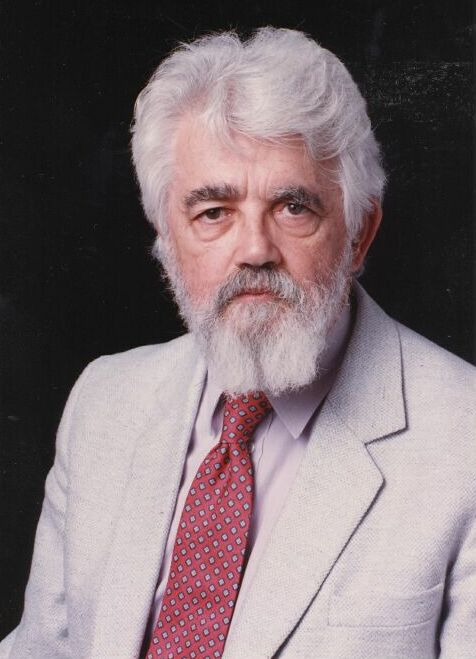
\includegraphics[height=0.3\textwidth]{img/mcCarthy.jpg}
    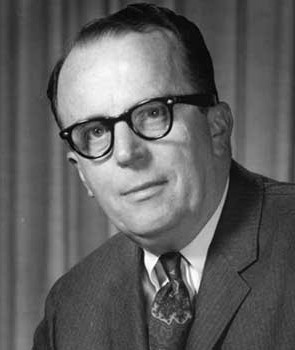
\includegraphics[height=0.3\textwidth]{img/licklider.jpg}
    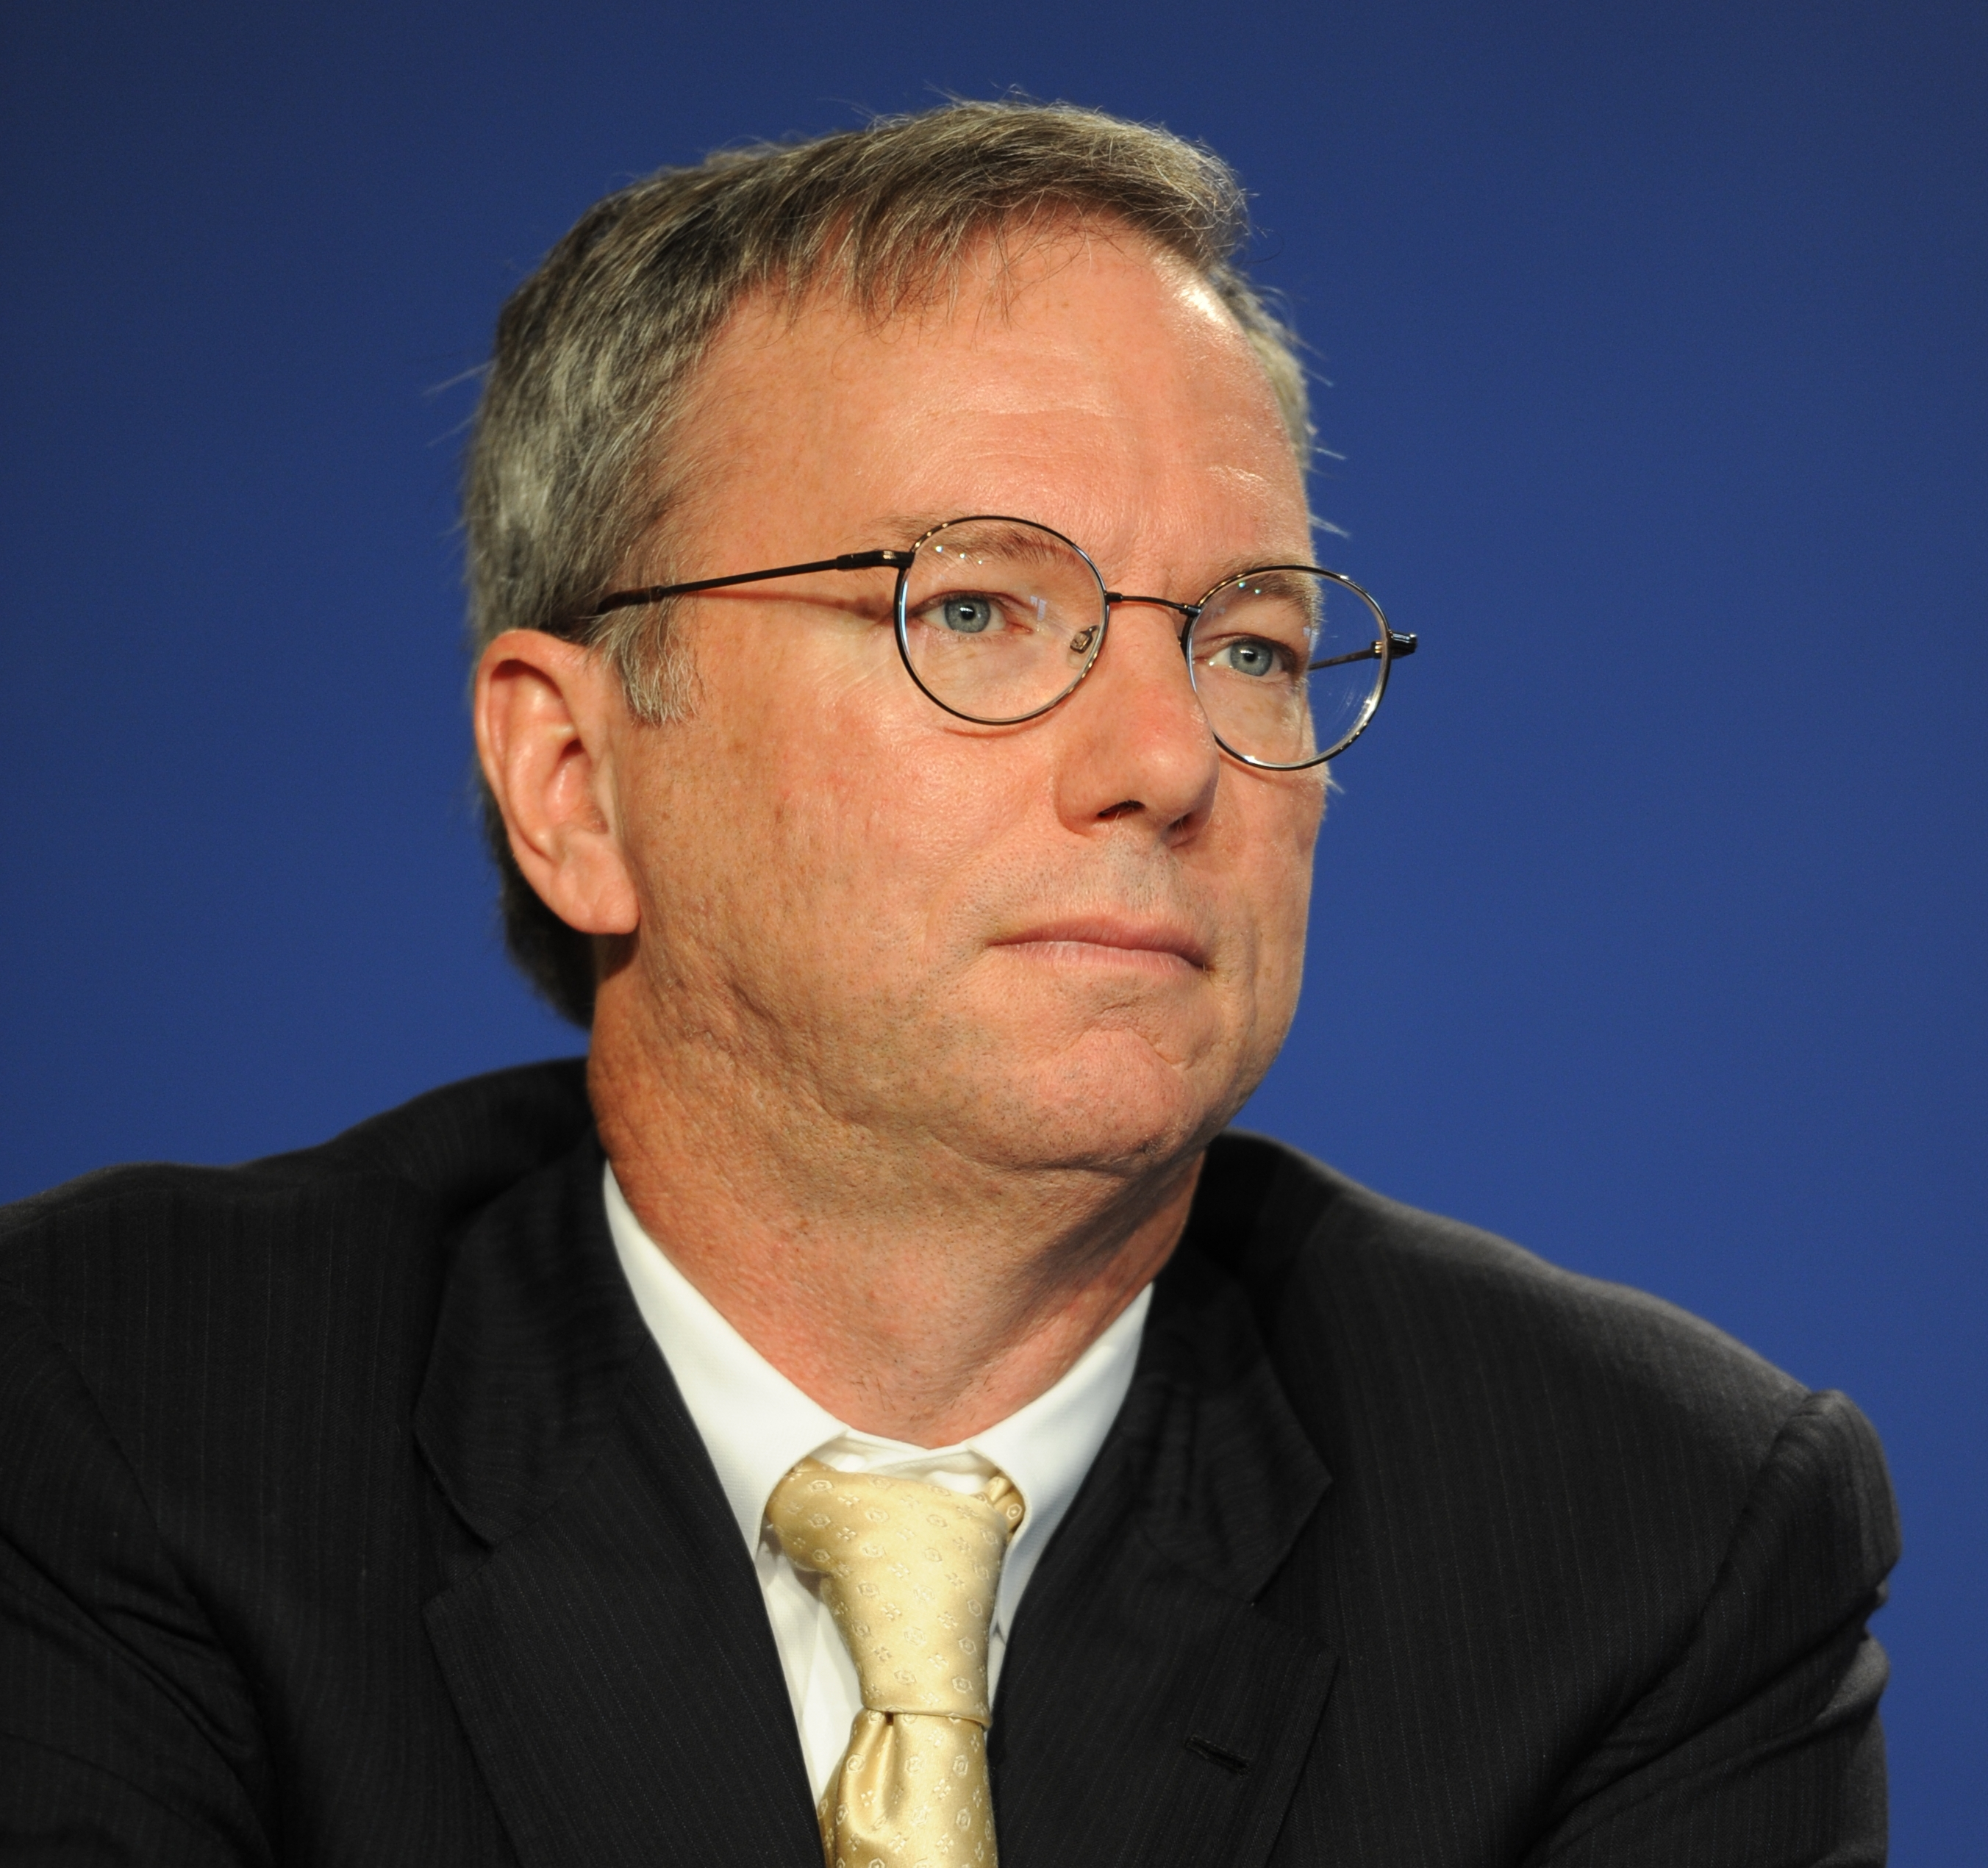
\includegraphics[height=0.3\textwidth]{img/schmidt.jpg}
    \caption{Da esquerda para a direta, John McCarthy~\cite{stanford-mccarthy-obit},
        J. C. R. Licklider~\cite{atimes-zoya-phantom} e Eric
        Schmidt~\cite{forbes-eric-schmidt:online}}
\end{figure}

% TODO: Mover, talvez, para a conclusão
% A computação em nuvem, até poucos anos atrás, era tida como uma tendência, mas hoje
% em dia é possível encontrar cada vez mais serviços que funcionam a partir de uma
% conexão com a Internet.

% Agora, fica a expectativa da evolução da computação em nuvem: por exemplo, será
% mesmo possível rodar todo um sistema operacional na nuvem? 
